\cm{Intro spiel}

\section{Molecule theory}
\label{theory:molecules}

\cm{
  \begin{itemize}
      \item Summary of basic energy structure: e-, vib, rot
      \item Making a MOT
      \item Microwave state selection
      \item Magnetic trapping
  \end{itemize}
}

\section{Chip trap theory}
\label{theory:chips}

% TODO Motivate chip traps in introduction
% TODO Set up with discussion of QP and IP traps including equations for their
% fields
In this section I will describe how a magnetic trap can be formed using
currents on the surface of a chip.

\subsection{Simple wire traps}

We begin our discussion by considering a simple case of a two-dimensional trap.
This will be formed of a straight wire carrying current $I$, which we
approximate to have infinite length. Such a wire can be free-standing or
deposited on a substrate.  The magnetic field due to the wire is described by
the Biot-Savart law~\cite{}, having magnitude
%
\begin{equation}
  B_w(r) = \frac{\mu_0 I}{2 \pi r}
\end{equation}
%
$r$ is the distance from the wire. The direction of the field obeys the right
hand rule. With such a geometry it is possible to create a ruidmentary
two-dimensional trap at a distance $h$ from the wire, by applying an external
bias field, whose direction opposes the field of the wire. To create the trap
at the desired bias, the strength of the field must be $\tilde{B}_y =
B(h)$~\cite{2011Ac}.

%TODO Use this notation in sim when descirbing calculation of the field!
Figure \myfigref{theory:fig:simplefield} illustrates this two-dimensional trap.
Here the wire oriented along the $x$ direction, with the current
$I=\SI{1}{\milli\ampere}$, flowing in the
positive direction (out of the page). This generates the expected field
$\mathbf{B}$ shown in subfigure (a). This is superimposed with the bias field
$\mathbf{\tilde{B}}_y$, also shown in (a), to produce the resulting field
$\mathbf{B} = \mathbf{B}_w + \mathbf{\tilde{B}}$ shown
in (b). This subfigure details the field lines (pink arrows), however these do
not tell the whole story, since weak-field seekers go to areas where the
magnitude of the field ($B$) is low. This is shown by the gradient, with darker
areas (blue, guide to the eye) indicating areas of lower field. The bias field
is chosen to induce a field minimum at $h=\SI{1}{\milli\meter}$. Subfigure (c)
shows a cut-through of the potential along $y$ with $x=0$, $z=h$. Subfigure (d)
also shows a cut-through of the potential along $z$ with $x=y=0$. This
demonstrates the two-dimensional trap.

\begin{figure}[htbp]
  \centering
  \begin{subfigure}[b]{0.45\textwidth}
    \centering
    \hfill{}
    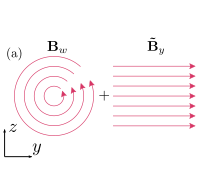
\includegraphics[width=0.8\textwidth]{figs/theory/wires/simplefield.pdf}
    \hfill{}
  \end{subfigure}
  \begin{subfigure}[b]{0.45\textwidth}
    \centering
    \import{figs/theory/wires/}{simpleheat_alone.pgf}
  \end{subfigure} \\
  \begin{subfigure}[b]{0.45\textwidth}
    \centering
    \import{figs/theory/wires/}{simpleheat_y.pgf}
  \end{subfigure}
  \begin{subfigure}[b]{0.45\textwidth}
    \centering
    \import{figs/theory/wires/}{simpleheat_z.pgf}
  \end{subfigure}
  \caption{
    The field from a simple two-dimensional wire trap. In subfigure (a) a wire carries
    current $I=\SI{1}{\milli\ampere}$ in the positive $x$ direction (out of the
    page) to create the usual field $\mathbf{B}_w$. This is combined with the
    external bias field $\mathbf{\tilde{B}}_y$ to create the two-dimensional trap
    at height $h=\SI{1}{\milli\meter}$
    shown in subfigure (b). The field lines are shown by pink arrows, and the
    magnitude of the resulting field is shown with the blue gradient (darker
    means weaker field, guide to the eye). Cut throughs of the potential are
    shown for $y$ (with $x=0$, $z=h$) in (c) and for $z$ (with $x = y = 0$) in
    (d).
  }
  \label{theory:fig:simplefield}
\end{figure}

Since the field minimum here is a zero, we can approximate the value near the
centre by a (two-dimensional) quadrupole with gradient
%
\begin{equation}
  B' = -\frac{2\pi \tilde{B}_y^2}{\mu_0 I}.
\end{equation}
%
The depth of the trap is $\mu \tilde{B}_y$, where $\mu$ is the \cm{magnetic dipole
moment} of the trapped particle. This can be seen in
\mysubfigref{theory:fig:simplefield}{d}: the potential is $B = |B_w(z) +
\tilde{B}_y|$, and so has an asymptote at $B=|\tilde{B}_y|$ as
$z\rightarrow\infty$.
%
We can transform such a trap into a Ioffe-Pritchard trap by applying a second
bias field along the $x$ direction to lift the field minimum away from
zero~\cite{2011Ac}.

Of course, it is commonly desirable to trap in all three dimensions. A simple
way to introduce confinement along the $x$ axis is to introduce a secocond wire
trap acting in the perpendicular direction. Such a device is called a dimple
trap (or cross conductor trap, or X-trap) and is illustrated in
\myfigref{theory:fig:dimple}. We label the current in the second wire $I_1$
and the new bias field, which is parallel to the $x$-axis and opposes the
$I_1$ field is labelled $\mathbf{B}_x$. In the case that $I_1 \ll I$, the
second wire can be treated as a perturbation of the first. The field minimum is
therefore still at $h$, and its depth is \cm{ref earlier equation?}.

\begin{figure}[htb]
    \centering
    \begin{tabular}[t]{cc}
\begin{subfigure}{0.3\textwidth}
    \centering
    \smallskip
    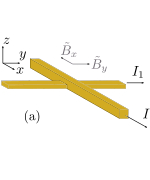
\includegraphics[width=\textwidth]{figs/theory/wires/dimple.pdf}
\end{subfigure}
    &
        \begin{tabular}{c}% if you add [t], than sub images are pushed down
        \smallskip
            \begin{subfigure}[t]{0.4\textwidth}
                \centering
                  \import{figs/theory/wires/}{dimpleheat_alone.pgf}
            \end{subfigure}\\
            \begin{subfigure}[t]{0.4\textwidth}
                \centering
                  \import{figs/theory/wires/}{dimple_x.pgf}
            \end{subfigure}
        \end{tabular}\\
    \end{tabular}
  \caption{
    The geometry of the dimple trap is shown in subfigure (a), with the new
    wire along $y$ carrying current $I_1$ intersecting the $I$ wire. An
    additional bias field in the $x$ direction, $\tilde{B}_x$ creates the field
    minimum. The field lines (pink) and magnitude (blue, darker is weaker,
    guide to the eye) is shown in subfigure (b) along $x=0$. Note the strong
    field region along the $y$ axis around the $I_1$ wire. Subfigure (c) shows
    a cut-through of the trapping potential in the $x$ direction with $y=0$,
    $z=h$.
  }
  \label{theory:fig:dimple}
\end{figure}

The dimple trap can be used as a quadrupole trap when the bias fields are
chosen to exactly cancel the magnetic field at the centre, or it can be used as
a Ioffe-Pritchard trap when there is a non-zero minimum. We will focus on the
latter case, in which case it is useful to write down the trap frequencies, the
derivation of which is similar to the one for the six-wire field discussed in
\cm{ref theory to be writtern}.
Since the trapping from the $I$ wire will be stronger than the $x$-axis
confinement from the $I_1 << I$ wire, we $\omega_x$ to be the weak trapping
direction. We again write down the field minimum
%
\begin{equation}
  B_0 = \left|\tilde{B}_x + \frac{\mu_0 I_1}{2\pi h}\right|,
\end{equation}
%
the transverse gradient
%
\begin{equation}
  B'_\perp = \frac{\mu_0 I}{2 \pi h^2},
\end{equation}
%
and the curvature along the weak component
%
\begin{equation}
  B'' = \frac{\mu I_1}{\pi h^3}.
\end{equation}
%
The trap frequency in the strong direction is~\cite{2011Ac}
%
\begin{equation}
  \omega_\perp = \sqrt{\frac{\mu B_\perp'^2}{m B_0}}
  \label{theory:eqn:perpfreq}
\end{equation}
%
where $m$ is the particle mass. In the weak direction (along $x$) the frequency
is~\cite{2011Ac}
%
\begin{equation}
  \omega_x = \sqrt{\frac{\mu B''}{m}}.
  \label{theory:eqn:xfreq}
\end{equation}

\subsection{The H-trap}

Consider the dimple trap, but with $\tilde{B}_x$ set to zero. Now what was
previously a magnetic field minimum will be a field maximum. By putting two
such dimple traps next to each other, it is possible to create a local minimum
within which we can trap molecules. Such a trap is called an H-trap, and is
pictured in \myfigref{theory:fig:Htrap}. We label the current due to the second
dimple trap $I_2$, and again note that the bias field in the $x$ direction can
be set to zero. The distance between $I_1$ and $I_2$ is denoted $d$, and we now
refer to the wire carrying current $I$ as the axis of the trap.

\begin{figure}[htb]
  \centering
  \begin{subfigure}[b]{0.4\textwidth}
    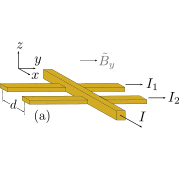
\includegraphics[width=\textwidth]{figs/theory/wires/Htrap.pdf}
    %\vspace{0.1mm}
  \end{subfigure}
  \begin{subfigure}[b]{0.4\textwidth}
    \import{figs/theory/wires/}{Hx.pgf}
  \end{subfigure}
  \caption{The geometry of the H-trap is shown in subfigure (a). In subfigure
  (b) we show the potential for an H-trap with
  $I_1=I_2=I/10=\SI{0.1}{\milli\ampere}$ and $d=\SI{10}{\milli\meter}$. Again the bias field is chosen so
  that $h=\SI{1}{\milli\meter}$.}
  \label{theory:fig:Htrap}
\end{figure}

We note that we need not choose $I_1$ and $I_2$ to be the same, although from
now on we will assume that they have the same magnitude, the sign can differ.
In other words the currents can be parallel or anti-parallel. In the former
case the trap forms a Ioffe-Pritchard trap; this is due to the fields from
$I_1$ and $I_2$ adding in the centre, to provide some overall non-zero
component in the $x$ direction. When the currents are anti-paraellel, the $I_1$
field opposes the $I_2$ field in the centre of the trap, the two cancel and
there is a field zero. Hence the latter configuration is a quadrupole trap.

In the Ioffe-Pritchard configuration, we can write down the field's
minimum~\cite{PhysRevA.79.013407}
%
\begin{equation}
  B_0 = \tilde{B}_x + 2\tilde{B}_y \frac{I-1}{I}\frac{h^2}{(d/2)^2 + h^2}
\end{equation}
%
transverse gradient~\cite{PhysRevA.79.013407}
%
\begin{equation}
  B'_\perp = \frac{2\pi\tidle{B}_y}{\mu_0 I}
\end{equation}
%
and curvature (in the $h \ll d$ limit)~\cite{PhysRevA.79.013407}
%
\begin{equation}
  B'' = \frac{12\tilde{B}_y I_1 h^2}{I (d/2)^4}
\end{equation}
%
and the trap frequencies are again given by equations~\ref{theory:eqn:perpfreq}
and~\ref{theory:eqn:xfreq}. In the quadrupole configuration, the traps is
characterised by the perpendicular gradient $B'_\perp$. 

\subsection{Three dimensinal single-wire traps}

Although the H-trap provides a method of creating a three dimensional
microtrap, it is not always convenient to have to use three distinct wires.
Fortunately the H-trap can be approximated by a single wire, either in a
U-shape for the quadrupole variant, or a Z-shape for the Ioffe-Pritchard
variant. These are pictured in \cm{theory:fig:HUZ}. Note that for the U-trap
the currents in the off-axis wires are once again anti-parallel, and in the
Z-trap these currents are parallel.

\begin{figure}[htb]
  \centering
  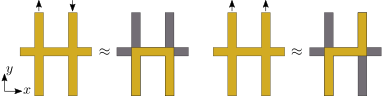
\includegraphics[width=\textwidth]{figs/theory/wires/HUZcomp.pdf}
  \caption{}
  \label{theory:fig:HUZ}
\end{figure}


\section{Quantum optics}
\label{theory:QO}

In this section we introduce a general model of molecules interacting with
light.  Since this is a broad field, I will focus the discussion only on the
details that are directly used in this thesis.  Namely the calculation of the
scattering rates for molecules in a light field and the coupling of molecules
to a light field in a resonator.

%\cm{Do I also need to discuss the normal mw spectroscopy in free space?}

\subsection{Scattering rates}

\cm{To come later}

\subsection{Cavity quantum electrodynamics}

A key part of the motivation for a molecule chip trap is the idea that
integrated microwave guides can be used to couple photons to the rotational
transitions of the molecules. Of particular interest is the idea
that a resonator can be used to perform this coupling, leading to the
ability to perform sideband-cooling to the motional ground state, state readout
and coupling between individually-trapped molecules~\cite{Andre2006}. This is
similar to techniques used in atom chips~\cite{Treutlein2008} and for optical
resonators coupling to atomic energy levels~\cite{SchleierSmith2011}.
% TODO Better cite in this last bit?

For our purposes, the coupling of a single molecule and the microwave field can
be treated as the coupling of a two-level system to a quantum mode of a cavity
field. The canonical description of such a system is given by the familiar
Jaynes-Cummings Hamiltonian (JCH) in the rotating wave
approximation~\cite{gerry_knight_2004}
%
\begin{equation}
  H_\text{JC} = \hbar\omega_c a^\dagger a + \frac{\hbar \omega_0}{2} \sigma_z +
  \frac{\hbar\Omega}{2}(a^\dagger \sigma_- + a\sigma_+)
  \label{theory:eqn:JCH}
\end{equation}
%
where $a$ ($a^\dagger$) is the annihilation (creation) operator of the photons,
$\Omega$ is the Rabi frequency of the interaction, $\sigma_i$ with $i\in{x, y,
z}$ are the Pauli matrices, and $\sigma_\pm =
(\sigma_x \pm i\sigma_y)/2$ are the raising and lowering operators of the
molecule state. The
detuning of the cavity resonance from that of the spin is $\Delta = \omega_0 -
\omega_c$. The system is shown in \mysubfigref{theory:fig:JCHstates}{a}.

\begin{figure}
  %\includegraphics{}
  \cm{Part (a) is image of JCH system, (b) is state manifold without coupling
  or detuning, (c) is state manifold with coupling (d) adds detuning (similar
  to Bohi fig 1)}
  \caption{\cm{TODO}}
  \label{theory:fig:JCHstates}
\end{figure}

We denote the ground (exicted) state of the molecule as $\ket{g}$ ($\ket{e}$).
The light field state can be taken to be a Fock state ($\ket{n}$ with $n \in
\mathbb{Z}$). Note that the final term in equation~\ref{theory:eqn:JCH}) has
the effect of exciting the ground state while absorbing a photon
($\ket{g}\ket{n} \leftrightarrow \ket{e}\ket{n-1}$) or lowering the excited state
and releasing a photon ($\ket{e}\ket{n} \leftrightarrow \ket{g}\ket{n+1}$).

Following the procedure in \inlineref{gerry_knight_2004}, we can see that this
mixing of the states results in a shift of the energy levels to create the
dressed states
%
\begin{align}
  \ket{+, n} &= \cos\Phi_n \ket{g}\ket{n} + \sin\Phi_n \ket{e}\ket{n+1} \\
  \ket{-, n} &= -\sin\Phi_n \ket{g}\ket{n} + \cos\Phi_n \ket{e}\ket{n+1}
\end{align}
%
with
%
\begin{equation}
  \tan(2\Phi_n) = \frac{\Omega\sqrt{n+1}}{\Delta}
\end{equation}
%
and having shifted energies
%
\begin{equation}
  E_{\pm, n} = (n+1)\hbar\omega_c \pm \frac{\hbar}{2}\sqrt{\Omega^2(n+1) +
  \Delta^2}.
  \label{theory:eqn:JCHenergies}
\end{equation}
%
It is useful to consider the manifold of states as depicted in
\myfigref{theory:fig:JCHstates}.  
%TODO This fig
Note that in the limit of no coupling
($\Omega = 0$) and no detuning ($\Delta = 0$) the energies are that of the bare
states, and $\ket{g}\ket{n+1}$ is degenerate with $\ket{e}\ket{n}$, as in part
(b) of the subfigure. Introducing coupling ($\Omega \neq 0$) lifts this
degeneracy, as in part (c). When the detuning is non-zero ($\Delta \neq 0$)
there is additional offset due to the second term in
\myeqref{theory:eqn:JCHenergies}, see part (d) of the figure.

The strong coupling r\'egime is reached when the coupling $g=2\Omega$ is
greater than the rate of decay from the cavity $\kappa = \omega_0 / Q$, where
$Q$ is called the quality factor of the cavity. The coupling parameter is
related to the transition dipole moment $d$ and the amplitude of the electric
field $E_0$ by
%
\begin{equation}
  \hbar g = \frac{d E_0}{2}.
\end{equation}
%
For the resonator, the amplitude of the electric field can be expressed in
terms of the cavity parameters by considering the electric field density
%
\begin{equation}
  \frac{1}{2} \epsilon_0 E_0 = \frac{\hbar \omega_0}{V}
\end{equation}
%
where $V$ is the volume of the mode in the cavity. The idea is to confine the
molecules in a trap that is on the $w=\SI{10}{\micro\meter}$ scale (see
chapter~\ref{overview}) and the resonator will necessarily have a length on the
scale of $\lambda_0 = 2\pi c / \omega_0$, therefore $V\approx w^2\lambda_0$.
Hence we have that
%
\begin{equation}
  g = \sqrt{\frac{2\pi c d^2}{\hbar \epsilon_0 w^2 \lambda_0^2}}.
\end{equation}

% TODO maybe move this whole sentence above
For the rotational \CaF{} transitions that we introduced above, in
section~\ref{theory:molecules} $d = \mu/\sqrt{3}$ with $\mu =
\SI{31}{\debye}$.
%
The coupling strength is therefore expected to be
%
% See nbs/2022-02-08_coupling.nb
\begin{equation}
  \frac{g}{2\pi} = \SI{20}{\kilo\hertz}
\end{equation}
%
and for strong coupling a cavity quality of
%
\begin{equation}
  Q = \frac{\omega_0}{g} > 1.7 \times 10^5
\end{equation}
%
is required.
